\chapter{Representation Formulas and Convolutions}

\setcounter{example}{1}
\setcounter{exercise}{1}

{\begin{center}
\psframebox[style=profibox]{\begin{minipage}{4in}
{\bf Prototype Question:} 
Find a formula for the solution of $\ddot{y} - 4 y = f(t)$, $y(0)=0)$, $\dot{y}(0)=0$ which can be evaluated to any desired accuracy for any given function $f(t)$.
\end{minipage}
}
\end{center}





In this section, we will write down several integral formulas for solutions of ODE.  These formulas are especially useful when it is difficult or impossible to write down closed form anti-derivatives.

Let us begin by considering the general first-order linear equation in standard form:
\[ \frac{dy}{dx}+p(x)y=q(x).\]
Suppose we seek a solution that satisfies the initial condition $y(x_0)=y_0$.  On a domain $I$ containing $x_0$ and where $p(x)$ and $q(x)$ are continuous, we would normally introduce any integrating factor of the form $\exp \left( \int p(x)dx \right)$.  However, let us now specify a particular anti-derivative as the argument of the exponential function (by taking advantage of the Fundamental Theorem of Calculus): we will use the integrating factor $\mu(x)=\exp \left( \int_{x_0}^x p(s)ds \right)$.
\[ \frac{d}{dx}\left[ \exp \left(\int_{x_0}^x p(s) ds \right) y \right] = q(x)\exp \left(\int_{x_0}^x p(s) ds \right).\]
And again, when we anti-differentiate both sides of this equation, we will use a particular anti-derivative on the right side:
\[ \exp \left( \int_{x_0}^x p(s) ds \right) y = C+\int_{x_0}^x q(t) \exp \left(\int_{x_0}^t p(s) ds \right)  dt. \]
(Note the presence of the constant of integration $C$ on the right side.)  
If we insert the initial condition at this point, notice that both definite integrals will be zero (since the upper and lower limits of integration will be identical), and we can see that $y_0=C$, so now we have
\[ \exp \left( \int_{x_0}^x p(s) ds \right) y = y_0+\int_{x_0}^x q(t) \exp \left(\int_{x_0}^t p(s) ds \right)  dt. \]
Isolating $y$ yields


{\begin{center}
\psframebox[style=formulabox]{\begin{minipage}{4.5in}
{\bf {\color{OliveGreen} Representation Formula for First-Order Linear Initial Value Problems \normalcolor}}

If $p(x)$ and $q(x)$ are continuous on an open interval $I$ containing $x_0$, then the unique solution of $y'+p(x)y=q(x)$ on $I$ is given by 
\[ y = \exp \left( -\int_{x_0}^x p(s) ds \right)  \left(y_0+\int_{x_0}^x q(t) \exp \left(\int_{x_0}^t p(s) ds \right) dt \right). \]
\end{minipage}
}
\end{center}



This is a representation formula that can be used for any first-order linear IVP in standard form.  The integrals are guaranteed to be defined on any domain where $p$ and $q$ are both continuous.  Even when we cannot write down an anti-derivative for the functions $p$ and $q$, we can often still write down approximate values of $y(x)$ by using a numerical method to approximate the integrals (such as the Trapezoid Rule, Simpson's Rule or another algorithm run by a calculator or computer.

\example Suppose $y$ satisfies the initial value problem $y'+2xy=1, \ y(0)=2$.  Find the approximate value of $y(1)$.

In theory the method of integrating factors will apply here, but we will run into some difficulty if we try actually calculate the exact solution because we will end up trying to anti-differentiate $e^{(x^2)}$, and there is no closed-form anti-derivative for this function.  However, we can apply the representation formula above (which is really just the method of integrating factors anyway) with $p(x)=2x$ and $q(x)=1$ to get
\begin{align*}
y(x) & = \exp \left( -\int_0^x 2s \ ds \right) \left( 2 + \int_0^x 1 \exp \left(\int_0^t 2s \ ds \right) dt \right) \\
& = e^{-(x^2)} \left( 2 + \int_0^x e^{(t^2)} \ dt \right)
\end{align*}
In particular,
\[ y(1) = e^{-1} \left( 2 + \int_0^1 e^{(t^2)} \ dt \right).\]
The integral on the right side can be calculated to any desired accuracy.  Simpson's Rule with $n=10$ subdivisions gives us $\int_0^1 e^{(t^2)} dt \approx 1.46268$.  Therefore $y(1) \approx 1.27385.$  (Careful use of the error estimate for Simpson's rule and careful rounding would allow us to conclude that the accuracy of this answer is better than  $10^{-4}$.)
\qed





\begin{exe} Use the above representation formula to write down a solution to $y'+xy=1$, $y(0)=1$.  Then give an approximate value of $y(2)$ by using a numerical method or computer to evaluate the definite integrals involved.
\end{exe}

Another representation formula can be obtained using the method of Laplace Transforms.  The key idea necessary is an operation on functions which is called convolution, so we must take a brief excursion to define this operation and examine some of its properties.

In pre-calculus we learn about several operations that combine functions.  The first few operations we explore are based on arithmetic: addition, subtraction, multiplication and division of functions.  Then we introduce a new operation that is different from what one has studied before: composition of functions.  Now will explore yet another way of combining functions which is of particular interest when working with Laplace Transforms.  This operation is defined in terms of definite integrals.

The 
	\index{convolution}%
	{\bf convolution} of two integrable functions $f$ and $g$ defined on $[0,\infty)$ is written as $f * g$ and is defined by the formula
\[ f*g (t) = \int_0^t f(\tau) g(t-\tau) \ d\tau.\]

\example Let $f(t)=t$ and $g(t)=e^t$.  Compute $f*g$.
\begin{align*}
f*g(t) & = \int_0^t f(\tau) g(t-\tau) \ d\tau \\
& = \int_0^t \tau e^{t-\tau} \ d\tau \\
& = e^t \int_0^t \tau e^{-\tau} \ d\tau \\
& = e^t \left( -\tau e^{-\tau} + \int e^{-\tau} \ d\tau \right)_0^t \\
& = e^t \left( -\tau e^{-\tau} -e^{-\tau} \right)_0^t \\
& = e^t(-t e^{-t} - e^{-t}+0+1) \\
& = -t-1+e^t.
\end{align*}
\qed

The first fact we will prove about convolution is that it is commutative: $f*g=g*f$.  Indeed,
\begin{align*}
f*g & = \int_{\tau=0}^{\tau=t} f(\tau)g(t-\tau) \ d\tau \\
& = -\int_{u=t}^{u=0} f(t-u)g(u) \ du \ \ \ \mbox{(substituting $u=t-\tau$)} \\
& = \int_{u=0}^{u=t}g(u)f(t-u) \ du \\
& = g*f.
\end{align*}
Therefore we need not specify the order of the two functions in a convolution.  

\begin{exe} 
Prove (by giving a counterexample) that the composition of functions $f \circ g$, defined by $(f \circ g)(x) = f(g(x))$, is not a commutative operation.
\end{exe}


\begin{exe} 
Find the convolution of the functions $t$ and $t^2$.
\end{exe}


Next, we examine what happens when we take the Laplace Transform of a convolution.
\begin{align*}
L[f*g] & = \int_0^\infty f*g(t) e^{-st} \ dt \\
& = \lim_{T \rightarrow \infty} \int_0^T \int_0^t f(\tau) g(t-\tau) e^{-st} \ d\tau \ dt \\
& = \lim_{T \rightarrow \infty} \int_0^T \int_\tau^T f(\tau) g(t-\tau) e^{-st} \ dt \ d\tau \ \ \ \ \ (*) \\
& = \lim_{T \rightarrow \infty} \int_0^T \int_0^{T-\tau} f(\tau)g(u)e^{-s(u+\tau)} \ du \ d\tau \\
& = \int_0^\infty \int_0^\infty f(\tau)g(u)e^{-s\tau}e^{-su} \ du \ d\tau \\
& = \left( \int_0^\infty f(\tau) e^{-s\tau} \ d\tau \right) \left( \int_0^\infty g(u) e^{-su} \ du \right) \\
& = (L[f])(L[g]).
\end{align*} 
In the line marked (*) we changed the order of integration, and the following figure illustrates how we obtained the new limits of integration:
\begin{center}
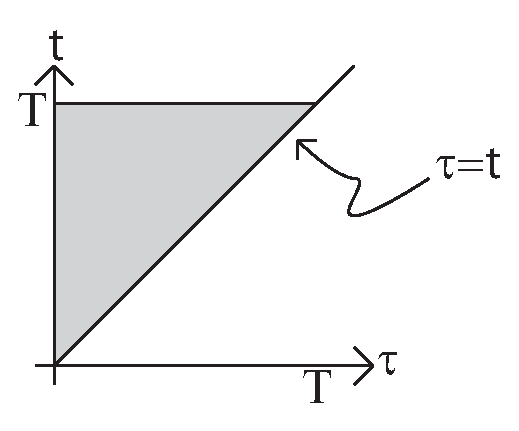
\includegraphics[width=2.5in]{12-representationformulas/convolutionfubini.eps}
\end{center}
What this result shows is that the Laplace Transform of a convolution of two functions is just the product of their Laplace Transforms.  This fact is valuable to us because it helps us to find more inverse transforms.


{\begin{center}
\psframebox[style=formulabox]{\begin{minipage}{4.5in}
{\bf {\color{OliveGreen} Laplace Transform of a Convolution \normalcolor}}
\index{convolution, Laplace transform of}

\[ L[f*g] = L[f]L[g].\]
Equivalently,
\[ L^{-1}[F(s)G(s)] = L^{-1}[F(s)] * L^{-1}[G(s)]. \]
\end{minipage}
}
\end{center}


\example The inverse Laplace Transform of $\frac{1}{(s-a)^2}$ is $te^{at}$ since
\begin{align*}
L^{-1} \left[ \frac{1}{s-a} \ \frac{1}{s-a} \right] & = L^{-1} \left[ \frac{1}{s-a}\right] * L^{-1} \left[ \frac{1}{s-a} \right] \\
& = e^{at} * e^{at} \\
& = \int_0^t e^{a\tau} e^{a(t-\tau)} \ d\tau \\
& = \int_0^t e^{at} \ d\tau \\
& = \left. \tau e^{at} \right|_0^t \\
& = te^{at}.
\end{align*}
\qed

\begin{exe}
Use the result of Example 3 above to solve the IVP $y''+10y'+25y=0, \ y(0)=1, \ y'(0)=2$ via Laplace Transforms.
\end{exe}

\begin{exe} 
Find $L^{-1} \left[ \frac{1}{s(s-1)} \right]$ two ways: (a) using convolutions and (b) using partial fractions.
\end{exe}





Now we have the necessary tool to develop more representation formulas.  

\example Find a formula for the solution of the initial value problem $\dot{y}+2y=f(t)$,  $y(0)=0$.  

Taking the Laplace Transform of each side of the differential equation produces
\[ L[\dot{y}+2y] = L[f],\]
so that
\[ s L[y]-y(0)+2L[y]=L[f],\]
and using the initial condition then isolating $L[y]$ yields
\[ L[y] = L[f]\frac{1}{s-1}.\]
If we know what $L[f]$ is, we might be able to evaluate this by hand, but only if we are able to look up the necessary inverse transforms in a table.  However, that is not necessary, because we come to this battle armed with convolutions!  Recall that $L[f*g]=L[f]L[g]$, and inverting that rule here with $g=L^{-1} \left[ \frac{1}{s-1} \right] = e^t$ gives us
\[ y = f(t) *e^t,\]
or
\[ y = \int_0^t f(\tau) e^{t-\tau} \ d\tau.\]
\qed

This formula can be applied even if we do not know the Laplace Transform of $f$.  For example, if $f(t)=\tan(t)$, and we want to know $y(0.5)$, then
\[ y(0.5) = \int_0^{0.5} \tan(\tau) e^{0.5 - \tau} \ d\tau = 0.155.\]
This approach gives us a numerical approximation, just like a technique such as Euler's Method would.  The advantage here is that we can obtain any desired accuracy provided we know how to approximate the necessary integral within the prescribed level of error.

\begin{exe}
Use Laplace Transforms and convolution to find an integral representation formula for $y(t)$ where $y$ satisfies the initial value problem $\dot{y} + 4y = \sec(t)$, $y(0)=0$, and use it to find an approximate value of $y(0.2)$.
\end{exe}

\begin{exe}
Use Laplace Transforms and convolution to find an integral representation formula for $y(t)$ where $y$  satisfies the initial value problem $\ddot{y}+4y = \cot(t)$, $y(0)=0$, $\dot{y}(0)=0$, and use it to find an approximate value of $y(0.3)$.
\end{exe}


\begin{exe}
Use Laplace Transforms and convolution to find an integral representation formula for $y(t)$ where $y$  satisfies the initial value problem $\ddot{y}-4\dot{y}+3y = e^{(t^2)}$, $y(0)=1$, $\dot{y}(0)=0$, and use it to find an approximate value of $y(0.2)$.
\end{exe}



%%% Cut below here for the book form.
%
%\newpage
%\begin{center} {\LARGE Problems} \end{center}
%
%\setcounter{problem}{1}




\newpage
\begin{center} {\LARGE Additional Exercises} \end{center}

\bigskip
\begin{multicols}{2}
\begin{instructions}
Write down an integral representation formula for the solution of the given initial value problem.  The use a graphing calculator or computer to evaluate the formula and approximate the value of $y(x_1)$.
\end{instructions}

\smallskip
\ap $y'+x^2y=1, \ y(0)=0, \ x_1 = 2$

\ap $y' + \sin(x) y = x, \ y(0)=0, \ x_1 = 1$

\ap $y' + \frac{y}{x} = e^{(x^4)}, \ y(0)=1, \ x_1 = 2$

\ap $y' - xy = x^2, \ y(0)=2, \ x_1 = 1$


\begin{instructions}
Calculate the given convolution of functions.
\end{instructions}

\smallskip
\ap $t^2 * t^2$

\ap $e^t * e^{2t}$

\ap $e^t * sin(t)$

\ap $cos(t) * cos(t)$


\begin{instructions} Use convolution to calculate the given inverse Laplace transform.
\end{instructions}

\smallskip
\ap $L^{-1} \left[ \frac{1}{(s-1)(s+1)} \right]$

\ap $L^{-1} \left[ \frac{1}{s(s+2)} \right]$

\ap $L^{-1} \left[ \frac{1}{s(s^2+1)} \right]$

\ap $L^{-1} \left[ \frac{1}{s^2(s^2+1)} \right]$

\begin{instructions} Use convolution to find an integral representation formula for the solution of the given initial value problem.
\end{instructions}

\smallskip
\ap $\ddot{y} = e^{(t^2)}, \ y(0)=0, \ \dot{y}(0)=0$

\ap $\ddot{y} + y = \tan(t), \ y(0)=0, \ \dot{y}(0)=0$

\ap $\ddot{y} - y = \cos(t^3), \ y(0)=0, \ \dot{y}(0)=0$

\ap $\ddot{y} -3\dot{y} + 2y = \sin(t^2), \ y(0)=0, \ \dot{y}(0)=0$


\smallskip
\hrule


\smallskip
\ap Use the method of integrating factors to find an integral representation formula for the solution of the following initial value problem with $b \neq 0$, and simplify your answer as much as possible:
\[ \dot{y}+by=f(t), \ y(0)=y_0.\]

\ap Use Laplace Transforms to find an integral representation formula for the solution of the following initial value problem with $b \neq 0$:
\[ \dot{y}+by=f(t), \ y(0)=y_0.\]

\ap Use Laplace Transforms to find an integral representation formula for the solution of the following initial value problem with $b \neq 0$:
\[ \ddot{y}+2b\dot{y}+b^2=f(t), \ y(0)=y_0, \dot{y}(0)=v_0.\]

\ap Use an integral representation formula to solve $\ddot{y}-y=f(t)$ with the initial conditions $y(0)=0$ and $\dot{y}(0)=0$.  Then let $f(t)=\ln(t-1)$, and estimate the value of $y(1)$ by evaluating the necessary definite integrals using Simpson's Rule.  Give an answer with an error less than $10^{-5}$.


\end{multicols}
